\subsection{Sistem Kontrol Adaptif dengan Model Prediktif berbasis \textit{Time Series}}

Seperti yang sudah dijelaskan pada bagian rancangan solusi (\ref{sec:rancangan-solusi}), sistem kontrol adaptif akan diimplementasikan dengan beberapa komponen penyusun, diantaranya adalah sebagai berikut.

\subsubsection{Komponen \textit{Metrics Fetcher}}
\textit{Metrics Fetcher} merupakan komponen yang berbeda dibanding komponen lainnya, karena komponen ini berjalan pada \textit{script} serta proses yang berbeda. Seperti yang sudah dijelaskan sebelumnya, komponen ini akan menembak permintaan HTTP pada \href{https://www.elastic.co/guide/en/elasticsearch/reference/current/cluster-nodes-stats.html}{\textit{Node Stats API}} yang telah disediakan \textit{Elastic Search} lalu melakukan transformasi bentuk data menjadi bentuk yang lebih sederhana dan sesuai kebutuhan. Komponen ini akan berjalan pada \textit{script} yang berbeda dikarenakan bahasa Python memiliki kekurangan dalam penanganan \textit{multithreading}. Komponen ini akan mengirimkan data yang sudah diolah ke komponen \textit{Predictor} melalui \textit{stream file}. Pendekatan ini dipilih karena sederhana dan mudah diimplementasikan. Khusus komponen ini, struktur kodenya tidak memakai sistem kelas dan hanya terdapat sebuah fungsi dan beberapa baris perintah untuk melakukan pemanggilan API, transformasi data dan pengiriman data ke \textit{stream file}.

\subsubsection{Komponen \textit{Predictor}}
Komponen \textit{Predictor} terdiri dari 3 buah kelas, yaitu sebagai berikut.
\begin{enumerate}
    \item \textbf{\textit{Predict Component}}
    
    Kelas ini berfungsi untuk menyimpan sebuah model ARIMA untuk sebuah variabel. Kelas ini memanfaatkan kakas pandas, statsmodels dan pmdarima untuk melakukan tanggung jawabnya.

    \item \textbf{\textit{Predict Component Factory}}
    
    Kelas ini berfungsi untuk membuat objek \textbf{\textit{Predict Component}} sebanyak variabel yang ada. 

    \item \textbf{\textit{Predict Component Storage}}
    
    Kelas ini berfungsi sebagai aggregator objek \textbf{\textit{Predict Component}} yang telah dibuat oleh \textbf{\textit{Predict Component Factory}}. Kelas ini juga berfungsi untuk meneruskan sebuah aksi kepada semua objek \textbf{\textit{Predict Component}} yang ada. Contohnya, dengan memanggil \textit{forecast} atau \textit{update data}, maka operasi akan diteruskan ke semua objek \textbf{\textit{Predict Component}}.

\end{enumerate}

\begin{figure}[h]
    \centering
    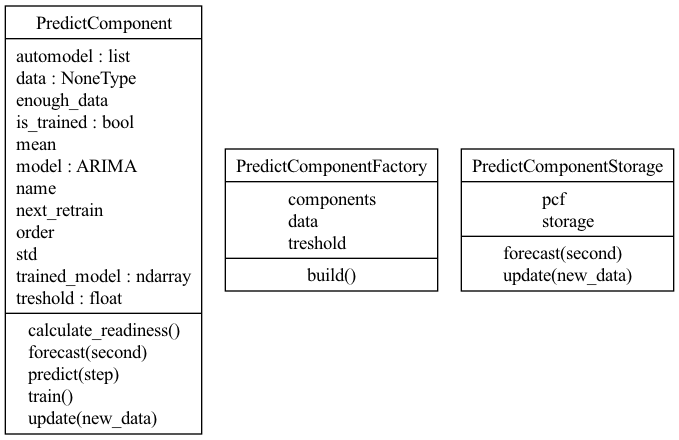
\includegraphics[width=0.8\textwidth]{chapter-4/predictor.png}
    \caption{Spesifikasi Kelas Penyusun Komponen \textit{Predictor}}
    \label{fig:predictor-spek}
\end{figure}

Secara umum, spesifikasi kelas bisa dilihat pada gambar \ref{fig:predictor-spek}. Kelas \textbf{\textit{Predict Component Storage}} akan membutuhkan \textbf{\textit{Predict Component Factory}} untuk membangun semua \textbf{\textit{Predict Component}} untuk setiap variabel yang ada. Setelah itu, terdapat operasi seperti meneruskan penambahan data serta meminta data prediksi ke setiap \textbf{\textit{Predict Component}}. Kelas ini akan digunakan oleh komponen \textit{Adaptive Control} untuk lebih lanjutnya.

\subsubsection{Komponen \textit{Rule Manager}}
Komponen \textit{Rule Manager} berfungsi untuk melakukan parsing terhadap file \textit{rule} yang telah diisi oleh pengguna serta menjadi aggregator untuk melakukan pengecekan \textit{rule} yang berlangsung serta memberi informasi data prediksi kapan saja yang dibutuhkan untuk melakukan pengecekan. Parsing komponen ini menggunakan format csv dan kondisi diekspresikan dengan sintaks python. Komponen ini akan menghasilkan sebuah objek \textit{Rule} yang akan digunakan oleh komponen \textit{Adaptive Control}. Agar terbayang, contoh dari \textit{file rule} dapat dilihat pada lampiran XXX. Spesifikasi dari kedua kelas tersebut dapat dilihat pada gambar \ref{fig:rule-spek}.

% TODO CONTOH RULE, masukin ke lampiran, trus tag kesini.

Sebuah \textit{rule} memiliki fungsi sebagai berikut.
\begin{enumerate}
    \item Memiliki sebuah kondisi yang akan dievaluasi dengan data prediksi pada waktu prediksi yang diinginkan. Contoh: kondisi \textit{throughput} untuk operasi X untuk 1 menit kedepan dan 5 menit kedepan lebih dari 1s, maka tingkatkan prosesor sebanyak 500m.
    \item Memiliki jumlah serta target kategori untuk diubah, dalam kasus ini pilihannya memori atau prosesor.
    \item Satuan untuk perubahan memori adalah dalam \textit{Mebibyte} atau MiB. Sedangkan untuk prosesor dalam satuan mili atau m.
    \item Sebuah \textit{rule} memiliki periode pengecekan sehingga tidak akan dicek secara terus menerus yang menyebabkan perubahan alokasi sumber daya terlalu cepat. Periode pengecekan dibuat dalam satuan sekon.
\end{enumerate}

\begin{figure}[h]
    \centering
    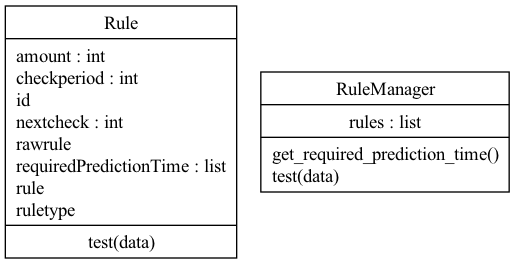
\includegraphics[width=0.8\textwidth]{chapter-4/rule.png}
    \caption{Spesifikasi Kelas Penyusun Komponen \textit{Rule Manager}}
    \label{fig:rule-spek}
\end{figure}

\subsubsection{Komponen \textit{Resource Controller}}

Komponen ini terdiri dari sebuah kelas. Seperti namanya, kelas ini berfungsi untuk menggunakan \textit{Kubernetes Client API} untuk mengubah alokasi sumber daya. Kelas ini diimplementasikan dengan sistem antrian, sehingga jika sejumlah rule aktif secara bersamaan, maka akan dijalankan secara berurutan. Terdapat sebuah fungsi \textit{tick} yang akan berfungsi untuk mengeksekusi antrian. Spesifikasi kelas ini dapat dilihat pada gambar \ref{fig:rc-spek}.

\begin{figure}[h]
    \centering
    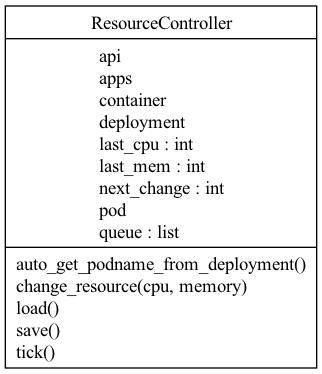
\includegraphics[width=0.8\textwidth]{chapter-4/rc.png}
    \caption{Spesifikasi Kelas Penyusun Komponen \textit{Resource Controller}}
    \label{fig:rc-spek}
\end{figure}

\subsubsection{Komponen \textit{Adaptive Control}}

\subsubsection{Tampilan Implementasi}